% =====================================================================
% INTERNET APPENDIX.
% Companion to "Mid-Ownership Concentration of the Literacy Moderation
% in the Momentum--Idiosyncratic-Volatility Anomaly: A Characterization
% Across States and Holders, 2009--2023."
% Compiles independently of main.tex; cross-references main.tex labels
% via xr-hyper.
% =====================================================================
\documentclass[12pt]{article}

\usepackage[utf8]{inputenc}
\usepackage[colorlinks=true,citecolor=blue,linkcolor=blue,urlcolor=blue]{hyperref}
\IfFileExists{papersetup.sty}{\usepackage{papersetup}}{}

\usepackage[margin=1in]{geometry}
\usepackage{setspace}
\onehalfspacing

\usepackage{amsmath}
\usepackage{amssymb}
\usepackage{amsthm}
\usepackage{mathtools}
\usepackage{natbib}
\usepackage{graphicx}
\usepackage{booktabs}

\usepackage{xr-hyper}
\externaldocument[][nocite]{../manuscript/main}

\title{Internet Appendix for\\ ``Locally Biased, Financially Blind: Where State Investor Literacy Moderates the Momentum--Idiosyncratic-Volatility Anomaly''}
\author{Adam Bozman}
\date{\today}

\begin{document}
\maketitle

\noindent This Internet Appendix collects the extended diagnostic material referenced in the main paper. The appendix is organized as a sequence of topical sections. Throughout, references of the form ``Table~\ref{tab:headline} of the main paper'' resolve to the labels in the main text.

\tableofcontents
\newpage

\appendix

\section{Point-in-time headquarters literacy reassignment: construction and full diagnostics}
\label{ia:pit}

This section records the construction of the EDGAR 10-K filing-header point-in-time (PIT) headquarters-state assignment and the full diagnostic stack on the PIT literacy reassignment that is the primary correctness check of Section~\ref{sec:nestedbaseline} of the main paper.

The canonical point-in-time headquarters location in the local-bias literature \citep{covalMoskowitz1999, pirinskyWang2006} is the business-address \texttt{STATE} in the Standard Generalized Markup Language header of a firm's SEC filings. For every panel firm with a Central Index Key (7,399 of 7,447 firms, linked permno-to-gvkey through the CRSP-Compustat link table and gvkey-to-CIK through the Compustat \texttt{company} file's \texttt{cik} field), I extract the business-address \texttt{STATE} from the SGML header of each in-sample 10-K filing 2009--2024. For 357 firms (older, longer-listed) the full sequence of in-sample 10-K headers was pulled, with median nine filings per firm; for the remaining 6,884 firms the first and last in-sample 10-K headers were fetched.

The PIT literacy reassignment re-merges each firm-month against the literacy distribution of the firm's then-current 10-K-header state (the most-recent 10-K filed at or before that month). The remerged \texttt{literacy\_z} is then re-z-scored within month. Coverage: 7,245 of 7,447 panel firms (97.3 percent) are PIT-covered; 1,370 firms have at least one PIT change relative to the static Compustat snapshot; 87,016 firm-months (13.95 percent of the panel) have a different headquarters state under PIT than under static; the PIT lookup misses 82 firm-months at the panel edges.

\begin{table}[h]
\centering
\caption{PIT literacy reassignment: aggregate three-way coefficient}
\footnotesize
\begin{tabular}{lrrr}
\toprule
Specification & $\hat\gamma$ & State-clustered $t$ (CR1) & wcb $p$ \\
\midrule
Static-snapshot full panel (baseline) & $-0.0117$ & $-2.17$ & $0.078$ \\
PIT literacy, PIT state cluster        & $-0.0003$ & $-0.86$ & $0.517$ \\
PIT literacy, static state cluster     & $-0.0003$ & $-0.64$ & $0.703$ \\
\bottomrule
\end{tabular}

\medskip
{\footnotesize\textit{Notes.} The PIT-state-cluster row clusters at the PIT (then-current) headquarters state; the static-state-cluster row clusters at the static Compustat snapshot to decompose the PIT-literacy effect from the PIT-clustering effect. Wild-cluster bootstrap uses Webb six-point weights, $B = 9{,}999$, null imposed.}
\end{table}

The PIT-literacy collapse is not a clustering artifact: changing the cluster dimension from PIT to static while keeping the PIT literacy merge leaves the coefficient unchanged at $-0.0003$. The collapse is driven by the literacy reassignment itself, not by the clustering scheme. Table~\ref{tab:nested} of the main paper reports the within-stock retail-versus-institutional difference under both merge conventions; the PIT collapse on the difference is consistent with the aggregate collapse here.

\section{Stable-headquarters subsample: construction and diagnostics}
\label{ia:stablehq}

The stable-headquarters subsample drops the 1,366 firms with a confirmed in-sample EDGAR 10-K-header relocation (Section~\ref{sec:stablehq} of the main paper). The flag construction uses two flags and unions them: \texttt{hdr\_changed} (10-K-header \texttt{STATE} changes across a firm's in-sample 10-Ks; 954 firms) and \texttt{sec\_disagree} (most-recent 10-K-header state disagrees with the static Compustat snapshot and the firm has at least two parsed 10-K headers; 524 additional firms). Coverage: 7,245 of 7,447 panel firms (97.3 percent) are flag-covered; the union identifies 1,366 unioned relocators (18.9 percent of flag-covered firms, 16.8 percent of firm-months).

The top first-to-last state pairs among \texttt{hdr\_changed} firms reproduce the documented corporate-relocation patterns of 2009--2024: New York to California (40 firms), California to Texas (37), New York to Texas (22), New York to Florida (21), California to Florida (18), New York to New Jersey (17). The flag is substantively credible and not picking up parsing noise.

The stable-headquarters subsample contains 519,090 firm-months and 6,081 firms. The full-panel mid-IO concentration table on the static-snapshot literacy merge is reported in Section~\ref{ia:fullpanelmidio} as a cross-check against Table~\ref{tab:headline} of the main paper.

\section{Within-retail IV-decile decomposition: full table}
\label{ia:ivdecile}

Section~\ref{sec:robust_battery} of the main paper summarizes the IV-decile decomposition of the within-retail wrong-signed literacy gradient on the persistent measure (five positive deciles, five negative; observation-weighted average $+0.0002$). This section reports the full table with within-decile state and permno counts.

\begin{table}[h]
\centering
\caption{IV-decile decomposition of the within-retail wrong sign: state and permno counts}
\footnotesize
\begin{tabular}{lrrrrrr}
\toprule
IV decile & DIFF persistent & wcb $p$ & DIFF time-varying & wcb $p$ & States (persist.) & Permnos \\
\midrule
0 & $-0.0005$ & $0.93$ & $+0.0009$ & $0.87$ & 41 & 201 \\
1 & $-0.0030$ & $0.41$ & $-0.0117$ & $0.013$ & 39 & 201 \\
2 & $+0.0021$ & $0.71$ & $+0.0109$ & $0.043$ & 40 & 200 \\
3 & $+0.0058$ & $0.16$ & $+0.0005$ & $0.91$ & 32 & 201 \\
4 & $-0.0053$ & $0.17$ & $+0.0055$ & $0.28$ & 38 & 200 \\
5 & $-0.0022$ & $0.60$ & $+0.0009$ & $0.80$ & 33 & 201 \\
6 & $+0.0032$ & $0.33$ & $-0.0016$ & $0.61$ & 34 & 200 \\
7 & $-0.0014$ & $0.70$ & $+0.0062$ & $0.057$ & 29 & 201 \\
8 & $+0.0071$ & $0.044$ & $+0.0024$ & $0.44$ & 30 & 200 \\
9 & $+0.0016$ & $0.86$ & $+0.0051$ & $0.47$ & 31 & 201 \\
\midrule
Obs-weighted avg & $+0.0002$ & --- & $+0.0013$ & --- & --- & --- \\
Pos / neg deciles & 5 / 5 & --- & 8 / 2 & --- & --- & --- \\
\bottomrule
\end{tabular}

\medskip
{\footnotesize\textit{Notes.} Each row re-estimates the stacked low-literacy-minus-high-literacy DIFF on the low-IO tercile of the stable-headquarters subsample, restricted to the within-month NYSE IV decile indicated. Wild-cluster bootstrap uses Webb six-point weights, $B = 4{,}999$. Sample: low-IO tercile of the stable-headquarters subsample, January 2009 through December 2023.}
\end{table}

\section{Mid-IO concentration on the full panel (static-snapshot literacy merge)}
\label{ia:fullpanelmidio}

Table~\ref{tab:headline} of the main paper reports the mid-IO concentration on the stable-headquarters subsample. For completeness, the same decomposition on the full panel under the static-snapshot literacy merge is reported here.

\begin{table}[h]
\centering
\caption{Mid-IO concentration on the static-snapshot full panel}
\footnotesize
\begin{tabular}{lcccc}
\toprule
Tercile & Persistent $\hat\gamma$ & State-clustered $t$ & Time-varying $\hat\gamma$ & State-clustered $t$ \\
\midrule
IO1 (low; high retail)        & $-0.0170$ & $-2.05$ & $-0.0118$ & $-1.66$ \\
IO2 (mid)                     & $-0.0185$ & $-2.14$ & $-0.0169$ & $-1.93$ \\
IO3 (high; institutional)     & $+0.0043$ & $+0.35$ & $+0.0060$ & $+0.41$ \\
\bottomrule
\end{tabular}

\medskip
{\footnotesize\textit{Notes.} The dependent variable is the monthly stock return; the coefficient is on the standardized three-way interaction within each IO tercile, on the full panel under the static-snapshot literacy merge. Sample: CRSP common stock, January 2009 through December 2023.}
\end{table}

On the static-snapshot full panel, both the low-IO and mid-IO terciles deliver state-clustered $|t|>2$ on the persistent IO measure; the high-IO tercile is small-positive. The mid-IO concentration of Table~\ref{tab:headline} of the main paper (where the low-IO coefficient attenuates relative to the mid-IO coefficient on the stable-headquarters subsample) is the result of restricting to stable-headquarters firms. The interpretation in Section~\ref{sec:mechanism} of the main paper engages the mid-IO concentration on the stable-headquarters subsample as the headline, because that is the population on which the channel family's theoretical unit of analysis is held fixed.

\section{PIT mid-IO under the literacy reassignment}
\label{ia:pitmidio}

For completeness, the PIT-literacy version of the mid-IO concentration table is reported here. Section~\ref{sec:robust_pit} of the main paper engages the magnitude collapse.

\begin{table}[h]
\centering
\caption{Mid-IO concentration under the PIT literacy reassignment (full panel)}
\footnotesize
\begin{tabular}{lcccc}
\toprule
Tercile & Persistent $\hat\gamma$ & State-clustered $t$ & Time-varying $\hat\gamma$ & State-clustered $t$ \\
\midrule
IO1 (low; high retail)        & $-0.00020$ & $-0.34$ & $+0.00008$ & $+0.17$ \\
IO2 (mid)                     & $-0.00121$ & $-2.07$ & $-0.00097$ & $-2.35$ \\
IO3 (high; institutional)     & $-0.00061$ & $-0.82$ & $-0.00085$ & $-1.34$ \\
\bottomrule
\end{tabular}

\medskip
{\footnotesize\textit{Notes.} As in Section~\ref{ia:fullpanelmidio}, on the full panel, but using the PIT literacy reassignment. The mid-IO coefficient is roughly a factor of 26 smaller in absolute value than under the stable-HQ static-literacy headline but is still the only tercile with state-clustered $|t| \geq 2$ on both IO measures. The directional pattern (mid-IO most negative, low-IO smallest) is preserved under PIT; the magnitude collapses.}
\end{table}

\section{20-bin quadratic-IO conditional-mean characterization}
\label{ia:quadbins}

Section~\ref{sec:headline} of the main paper reports the quadratic-IO continuous-margin four-way result and its implied $\mathrm{IO}^* \approx 0.30$ interior minimum. This section reports the 20-bin conditional-mean characterization of the three-way slope across the IO distribution that corroborates the U-shape independently. The persistent IO measure is partitioned into 20 IO percentile bins on the full panel; within each bin, the three-way slope is estimated by residualizing on the lower-order interactions and the fixed effects and then taking the within-bin OLS slope.

\begin{table}[h]
\centering
\caption{20-bin conditional-mean three-way slope across the IO distribution}
\footnotesize
\begin{tabular}{lrrr}
\toprule
IO bin & IO percentile range & IO share mean & Conditional three-way slope \\
\midrule
1 & 0.00--0.05 & 0.019 & $-0.00089$ \\
2 & 0.05--0.10 & 0.050 & $+0.00004$ \\
3 & 0.10--0.15 & 0.088 & $-0.00112$ \\
4 & 0.15--0.20 & 0.136 & $-0.00083$ \\
5 & 0.20--0.25 & 0.187 & $+0.00150$ \\
\textbf{6} & \textbf{0.25--0.30} & \textbf{0.244} & $\mathbf{-0.00463}$ \\
7 & 0.30--0.35 & 0.299 & $+0.00080$ \\
8 & 0.35--0.40 & 0.356 & $+0.00147$ \\
9 & 0.40--0.45 & 0.410 & $-0.00195$ \\
10 & 0.45--0.50 & 0.458 & $-0.00147$ \\
11 & 0.50--0.55 & 0.500 & $-0.00162$ \\
12 & 0.55--0.60 & 0.539 & $+0.00024$ \\
13 & 0.60--0.65 & 0.575 & $-0.00243$ \\
14 & 0.65--0.70 & 0.606 & $+0.00052$ \\
15 & 0.70--0.75 & 0.638 & $-0.00159$ \\
16 & 0.75--0.80 & 0.666 & $+0.00091$ \\
17 & 0.80--0.85 & 0.696 & $+0.00170$ \\
18 & 0.85--0.90 & 0.726 & $+0.00041$ \\
19 & 0.90--0.95 & 0.763 & $+0.00038$ \\
20 & 0.95--1.00 & 0.832 & $+0.00097$ \\
\bottomrule
\end{tabular}

\medskip
{\footnotesize\textit{Notes.} Within each persistent-IO percentile bin on the full panel, the residualized three-way slope is the within-bin OLS slope of $r_{i,s,t}$ on the standardized $\mathrm{mom}\times\mathrm{IV}\times\mathtt{literacy\_z}$ term after residualizing on the lower-order interactions, state fixed effects, and month fixed effects. Bin 6 (bold) is the most-negative bin (IO share mean 0.244), approximately ten percentage points below the parametric quadratic-IO trough $\mathrm{IO}^{\ast} \approx 0.34$ of Section~\ref{sec:quadratic} of the main paper; bin 17 (IO share mean 0.696) is the most-positive bin.}
\end{table}

The most-negative bin lies at IO percentile 25--30 (IO share mean 0.244), below the parametric quadratic trough at $\mathrm{IO}^{\ast} \approx 0.34$. The 20-bin diagnostic is non-parametric corroboration of an interior minimum but does not match the parametric trough location precisely; the average over the two endpoint bins is $+0.00004$ (zero), and the mildly positive bins above IO percentile 80 are consistent with a U-shape opening upward.

\section{Relocator-vs-stable-HQ characteristics comparison}
\label{ia:relocchar}

The 1,366 relocator firms dropped from the stable-HQ subsample are not a random sample of the full panel. Table~\ref{tab:reloc_char} reports the firm-mean comparison between the 1{,}366 relocators and the 6{,}081 retained stable-HQ firms with Welch $t$-statistics on the difference.

\begin{table}[h]
\centering
\caption{Relocator-vs-stable-HQ firm-mean characteristics}
\label{tab:reloc_char}
\footnotesize
\begin{tabular}{lrrrrr}
\toprule
Characteristic & Relocator mean (SD) & Stable mean (SD) & Difference & Welch $t$ & $p$ \\
\midrule
Market cap (\$M)                & 2{,}138 (9{,}144) & 3{,}623 (12{,}453) & $-1{,}485$ & $-5.04$ & $<0.001$ \\
Log market cap                  & 5.37 (1.94)       & 5.90 (2.13)        & $-0.53$    & $-8.95$ & $<0.001$ \\
Idiosyncratic volatility (z)    & $+0.477$ (0.843)  & $+0.133$ (0.852)   & $+0.345$   & $+13.63$ & $<0.001$ \\
Momentum (12-2)                 & $-0.277$ (0.612)  & $-0.069$ (0.590)   & $-0.209$   & $-11.46$ & $<0.001$ \\
IO share (persistent)           & 0.378 (0.259)     & 0.454 (0.245)      & $-0.076$   & $-9.83$  & $<0.001$ \\
Monthly return                  & $-0.0073$ (0.051) & $+0.0102$ (0.056)  & $-0.018$   & $-11.33$ & $<0.001$ \\
\texttt{literacy\_z}            & $-0.063$ (0.837)  & $+0.040$ (0.800)   & $-0.103$   & $-4.15$  & $<0.001$ \\
\bottomrule
\end{tabular}

\medskip
{\footnotesize\textit{Notes.} Firm-mean of each characteristic computed over the firm's in-sample firm-months, then averaged across firms in each group. Relocators are the 1{,}366 firms with a confirmed in-sample EDGAR 10-K-header relocation (union of \texttt{hdr\_changed} and \texttt{sec\_disagree}); stable-HQ are the 6{,}081 retained firms. Welch $t$-statistic on the difference of means.}
\end{table}

Relocators are systematically smaller (market cap roughly 60 percent of stable-HQ), higher-IV (idiosyncratic volatility z-score 3.6 times larger), more negative-momentum, lower-IO, lower-return, and from slightly lower-literacy states. Every characteristic differs at $t > 4$. The systematic selection is consistent with relocators being firms whose corporate-strategy decisions (including headquarters moves) place them in a different segment of the cross-section than the community-anchored, larger, lower-IV firms that constitute the stable-HQ population. The relocator profile is plausibly mechanism-relevant: smaller, high-IV, lower-literacy-state firms whose corporate-strategy headquarters changes are themselves correlated with the local-anchored channel breaking down.

Section~\ref{sec:relocator} of the main paper engages the relocator decomposition of the headline mid/low ratio; Section~\ref{sec:robust_pit} engages the PIT-vs-stable-HQ magnitude collapse on the mid-IO coefficient and notes that the design does not separate the mechanism-strength reading from the sample-selection reading.

\section{Refined-relocator stable-headquarters extension}
\label{ia:refinedreloc}

The headline stable-headquarters subsample of Section~\ref{sec:headline} of the main paper drops 1,366 firms under the union of \texttt{hdr\_changed} and \texttt{sec\_disagree}. A narrower refinement using only \texttt{hdr\_changed} (dropping 954 firms, retaining the 412 firms where the SEC-Compustat disagreement is the only flag) defines the refined-relocator subsample. On the refined-relocator subsample under the static-snapshot literacy merge, the stacked low-IO-minus-high-IO difference is $-0.0146$ persistent (wcb $p = 0.36$) and $-0.0110$ time-varying ($p = 0.55$), larger in absolute value than on the broad stable-headquarters subsample of Table~\ref{tab:headline} of the main paper but still inferentially weak.

\section{Full inference battery on the static-snapshot aggregate}
\label{ia:inference}

This section reports the detail behind the aggregate inference on the static-snapshot full panel (Section~\ref{sec:nestedbaseline} of the main paper, Panel A first row). The headline inference procedure is the state-level wild-cluster bootstrap of \citet{cameronGelbachMiller2008}, run with Webb six-point weights, the null imposed, and $B = 9{,}999$ replications. It returns $p = 0.078$, a 95-percent studentized bootstrap confidence interval of $[-0.0250, +0.0017]$, and a 95-percent percentile interval of $[-0.0223, -0.0014]$. The two-way Cameron-Gelbach-Miller (2011) state-by-month clustered standard error is 0.0022, against a one-way state-clustered standard error of 0.0055; the ratio of 2.5 is why the two-way clustered $t = -5.32$ over-states the evidence relative to the wild-cluster bootstrap. The block bootstrap on the Fama-MacBeth coefficient returns $p = 0.396$, and the Romano-Wolf family-wise $p$-value of 0.676 is computed across the four pre-registered implications using the stepwise procedure of \citet{romanoWolf2005}.

\section{Inference-divergence diagnosis: leverage detail}
\label{ia:divergence}

The full jackknife-by-month detail for the aggregate three-way on the static-snapshot full panel is as follows.

\begin{table}[h]
\centering
\caption{Leverage analysis: dropping high-influence months and calendar years}
\footnotesize
\begin{tabular}{lrrr}
\toprule
Specification & Coefficient & $t$-statistic & $N$ \\
\midrule
Full sample                       & $-0.0117$ & $-5.32$ (CGM)       & 623,896 \\
Drop top-5 influence months        & $-0.0131$ & $-2.42$ (state-CR1) & 606,068 \\
Drop top-10 influence months       & $-0.0145$ & $-2.69$ (state-CR1) & 589,411 \\
Drop calendar-2009                 & $-0.0086$ & $-4.07$ (CGM)       & --- \\
Drop calendar-2020                 & $-0.0149$ & $-3.36$ (CGM)       & --- \\
Drop calendar-2009 and 2020        & $-0.0121$ & $-2.58$ (CGM)       & --- \\
\bottomrule
\end{tabular}
\end{table}

\noindent The largest single-month influence is 14.8 percent of the full-sample coefficient. The pooled estimate on the static-snapshot full panel is not an artifact of the 2009 recovery or the 2020 shock.

\section{Subsample stability: full five-window grid}
\label{ia:subsample}

Table~\ref{tab:prepost_grad} (Section~\ref{ia:prepost}) reports the pre-2015 and post-2015 split. This section reports the full five-window grid for the headline Fama-MacBeth estimator on the static-snapshot full panel.

\begin{table}[h]
\centering
\caption{Five-window subsample grid, Fama-MacBeth Newey-West estimator, static-snapshot full panel}
\footnotesize
\begin{tabular}{lrrrr}
\toprule
Window & Coefficient & SE & $t$-statistic & Months \\
\midrule
Full (2009--2023)        & $-0.00599$ & $0.00705$ & $-0.85$ & 180 \\
Pre-2015                 & $-0.01845$ & $0.01019$ & $-1.81$ & 72 \\
Post-2015                & $+0.00232$ & $0.00836$ & $+0.28$ & 108 \\
Pre-COVID ($<$2020-03)   & $-0.00776$ & $0.00828$ & $-0.94$ & 134 \\
Post-COVID               & $-0.00083$ & $0.01174$ & $-0.07$ & 46 \\
\bottomrule
\end{tabular}
\end{table}

\section{Alternative literacy constructions}
\label{ia:altlit}

This section reports the Fama-MacBeth estimator on the static-snapshot full panel under six alternative constructions of the literacy variable, for both the contemporaneous return and the one-month-lead return.

\begin{table}[h]
\centering
\caption{Alternative literacy proxies, Fama-MacBeth Newey-West estimator, static-snapshot full panel}
\footnotesize
\begin{tabular}{lrrrr}
\toprule
Literacy proxy & Coefficient & SE & $t$-statistic & Months \\
\midrule
\multicolumn{5}{l}{\textit{Panel A: Contemporaneous return}}\\
Continuous z-score (headline)        & $-0.00599$ & $0.00705$ & $-0.85$ & 180 \\
Mean Big Five score                  & $+0.00021$ & $0.00034$ & $+0.61$ & 180 \\
Share scoring $\geq 4/5$             & $-0.00054$ & $0.00042$ & $-1.28$ & 180 \\
Percentile rank                      & $-0.00008$ & $0.00037$ & $-0.23$ & 180 \\
Low-literacy dummy                   & $-0.00016$ & $0.00041$ & $-0.38$ & 180 \\
Lag-36 EIV-instrumented              & $-0.00007$ & $0.00031$ & $-0.23$ & 144 \\
\midrule
\multicolumn{5}{l}{\textit{Panel B: One-month-lead return}}\\
Continuous z-score                   & $+0.00615$ & $0.00627$ & $+0.98$ & 179 \\
Mean Big Five score                  & $+0.00060$ & $0.00034$ & $+1.74$ & 179 \\
Share scoring $\geq 4/5$             & $-0.00018$ & $0.00030$ & $-0.60$ & 179 \\
Percentile rank                      & $+0.00044$ & $0.00034$ & $+1.29$ & 179 \\
Low-literacy dummy                   & $-0.00055$ & $0.00037$ & $-1.49$ & 179 \\
Lag-36 EIV-instrumented              & $-0.00011$ & $0.00043$ & $-0.26$ & 143 \\
\bottomrule
\end{tabular}
\end{table}

\section{Herfindahl-Hirschman alternative}
\label{ia:hhi}

Replacing IO terciles with terciles on the institutional Herfindahl-Hirschman index of 13F-manager shares (canonical HHI proxy $1/n_{\text{mgr}}$ at the firm-quarter level), Table~\ref{tab:hhi_ia} reports the three-way coefficient per HHI tercile on the stable-HQ subsample.

\begin{table}[h]
\centering
\caption{HHI-tercile three-way coefficients, stable-HQ subsample}
\label{tab:hhi_ia}
\footnotesize
\begin{tabular}{lcccr}
\toprule
HHI tercile ($1/n_{\text{mgr}}$) & $\hat\gamma$ & State-$t$ & $N$ \\
\midrule
HHI1 (low concentration; high $n_{\text{mgr}}$)  & $-0.0296$ & $-1.52$ & 264,927 \\
HHI2 (mid)                                       & $-0.0135$ & $-1.40$ & 145,768 \\
HHI3 (high concentration; low $n_{\text{mgr}}$)  & $-0.0138$ & $-0.98$ & 108,267 \\
\midrule
\multicolumn{4}{l}{Mid-HHI / low-HHI ratio $= 0.46$ (vs. mid-IO / low-IO $= 2.83$).} \\
\bottomrule
\end{tabular}

\medskip
{\footnotesize\textit{Notes.} The three-way coefficient within each HHI tercile of the stable-HQ subsample. HHI terciles are formed on each firm's time-mean $1/n_{\text{mgr}}$ in the Thomson Reuters s34 panel. State-clustered $t$-statistics.}
\end{table}

The mid-HHI/low-HHI ratio is $0.46$, very different from the mid-IO/low-IO ratio of $2.83$. The HHI margin does not mirror the IO-share margin. An IO-share channel does not transmit through HHI for a structural reason: the IO-share margin tracks the level of institutional presence in a stock (the population proportion against which the literacy-modulated retail demand is netted) while HHI tracks how concentrated that institutional presence is across managers. A literacy-modulated retail demand on a stock with low institutional presence in aggregate behaves the same whether the few institutions present are concentrated or dispersed. The HHI null is therefore not evidence against any ownership-concentration channel; it shows that the documented contrast is about ownership level rather than ownership concentration.

\section{Classical errors-in-variables: per-wave reliability detail}
\label{ia:eiv}

Section~\ref{sec:discussion} of the main paper reports the firm-month-weighted reliability ratio $\lambda = 0.420$ and the EIV-corrected mid-IO coefficient. Table~\ref{tab:eiv_ia} reports the per-wave reliability ratios.

\begin{table}[h]
\centering
\caption{Per-wave NFCS reliability ratios}
\label{tab:eiv_ia}
\footnotesize
\begin{tabular}{lccc}
\toprule
NFCS wave & cross-state $V(\hat p)$ & mean $V(\text{err})$ & $\lambda_{w}$ \\
\midrule
2009 & 0.000492 & 0.000388 & 0.211 \\
2012 & 0.000772 & 0.000404 & 0.476 \\
2015 & 0.000612 & 0.000392 & 0.359 \\
2018 & 0.000836 & 0.000367 & 0.562 \\
2021 & 0.000754 & 0.000364 & 0.517 \\
\midrule
Firm-month-weighted $\lambda$ & \multicolumn{3}{c}{$0.420$} \\
\bottomrule
\end{tabular}

\medskip
{\footnotesize\textit{Notes.} Per-wave reliability ratio $\lambda_{w} = V_{\text{true}}/V_{\text{obs}} = (V_{\text{obs}} - V_{\text{err}})/V_{\text{obs}}$, where $V_{\text{obs}}$ is the cross-state variance of the wave's state-level NFCS Big-Five share-correct estimate and $V_{\text{err}}$ is the mean sampling variance $\hat p(1-\hat p)/n_{\text{eff}}$. An earlier draft used an empirical-Bayes shrinkage which on independent verification traced to a normalization artifact (within-month correlation between raw and shrunk literacy $> 0.99$); classical EIV is the theoretically principled treatment and replaces the shrinkage. Under alternative correct-EB reconstructions that preserve the panel's z-scoring topology, the same regressor delivers $\hat\beta \in [-0.0083, -0.0077]$ with $p \approx 0.45$; classical EIV is the principled point.}
\end{table}

\section{Korniotis-Kumar business-cycle block: one- and two-proxy detail}
\label{ia:kk}

Adding the state unemployment rate and the Philadelphia Fed coincident-index growth rate (each z-scored within month and interacted with momentum, IV, and $\mathrm{mom}\times\mathrm{IV}$) to the static-snapshot full panel attenuates the aggregate three-way: the one-proxy block (state unemployment) retains 76.6 percent of the raw coefficient magnitude, moving $\hat\gamma$ from $-0.01173$ to $-0.00898$; the two-proxy block retains 80.1 percent, moving $\hat\gamma$ from $-0.01177$ to $-0.00943$ (the two-proxy sample is slightly smaller). The coefficient remains negative under two-way Cameron-Gelbach-Miller clustering in both. The 20--23 percent attenuation is a lower bound on business-cycle overlap; sophistication-beyond-business-cycle is the residual economic content. The pre/post-2015 split of the one-proxy block is $-0.01585$ ($t = -1.32$) pre-2015 and $-0.00780$ ($t = -2.41$) post-2015.

\section{The Thomson Reuters s34 institutional-ownership panel}
\label{ia:thomson}

This section records the construction of the canonical institutional-ownership panel. The source is the WRDS Thomson Reuters s34 13F holdings file, pulled for all 60 calendar quarters from 2009Q1 through 2023Q4: 222,180 firm-quarter observations across 7,907 distinct permnos.

The numerator is the literature-standard amendment-deduplicated sole-plus-shared institutional-share construction. Amendment-deduplication keeps only the latest filing per (manager, security, report-date) triple via \texttt{DISTINCT ON (mgrno, cusip) ORDER BY fdate DESC}; sole-plus-shared is the institutional-share numerator. The two corrections are jointly required: amendment-deduplication alone (with raw \texttt{shares}) leaves 5.73 percent of firm-quarters above one, and sole-plus-shared alone (without amendment-deduplication) does not address the amendment-stacking; the two together bring the above-one rate to 0.36 percent.

For each issuer cusip and report date, sole-plus-shared shares are summed across amendment-deduplicated 13F managers; cusip is matched to permno through the CRSP \texttt{stocknames} historical-cusip file valid at the report date; the sample is restricted to common equity (share codes 10 and 11). The shares-outstanding denominator is CRSP \texttt{msf} \texttt{shrout} at the report-date month-end. The 0.36-percent residual above-one rate is the irreducible cross-manager shared-block measurement-noise floor and is capped at one.

The persistent measure is each firm's time-mean share across its available Thomson quarters; the time-varying measure assigns each firm-month the share from the most recent 13F quarter whose report date is at least four months earlier (no look-ahead). Sample coverage by panel and measure is reported in Table~\ref{tab:descriptives} (Panel B) of the main paper.

\section{EDGAR-proxy cross-check of the ownership split}
\label{ia:edgar}

Before WRDS access to the Thomson Reuters s34 panel was available, an earlier draft of this paper built the institutional-ownership split from a partial EDGAR 13F parse. The EDGAR proxy was constructed from raw Form 13F-HR filings retrieved from the SEC EDGAR system: for each filing, the holdings infotable was parsed, share-type positions kept and option positions excluded, institutional shares aggregated by ticker, and the total divided by shares outstanding. The parse covered six quarters between 2009Q2 and 2021Q2; the raw share exceeded one for 21.7 percent of matched firm-quarters, reflecting ticker-match collisions and multi-class-share double-counting that the cusip-level Thomson construction largely resolves. On the EDGAR-proxy persistent measure on the static-snapshot full panel, the low-minus-high ownership difference is $-0.043$ with a state-level wild-cluster bootstrap $p$ of 0.021. The directional pattern under the static-snapshot merge reproduces on the EDGAR proxy. The canonical Thomson panel under the literature-standard numerator is the arbiter; the EDGAR proxy is a cross-check.

\section{Within-retail literacy-gradient detail}
\label{ia:withinretail}

This section records the detail behind the within-retail literacy gradient of Section~\ref{sec:robust_battery} of the main paper. On the persistent IO measure of the stable-headquarters subsample, within the low-IO tercile: $\hat\gamma$ in high-literacy states is $+0.0060$ (state-clustered $t = +0.32$, $n = 88{,}034$, 25 states); $\hat\gamma$ in low-literacy states is $+0.0094$ ($t = +0.71$, $n = 56{,}955$, 25 states); the stacked low-literacy-minus-high-literacy DIFF is $+0.0033$ (state-clustered $t = +2.80$, wild-cluster bootstrap $p = 0.024$, 95-percent studentized interval $[+0.00044, +0.00599]$, $B = 4{,}999$).

On the time-varying IO measure of the stable-headquarters subsample, within the low-IO tercile: $\hat\gamma$ in high-literacy states is $+0.0054$ ($t = +0.34$, $n = 87{,}354$, 26 states); $\hat\gamma$ in low-literacy states is $+0.0090$ ($t = +0.75$, $n = 53{,}775$, 25 states); the stacked DIFF is $+0.0029$ ($t = +2.00$, wild-cluster bootstrap $p = 0.093$, 95-percent studentized interval $[-0.0006, +0.0063]$).

\section{Median-split tie-resolution rule and within-tercile cluster counts}
\label{ia:medsplit}

The within-retail literacy split summarized in Section~\ref{sec:robust_battery} of the main paper splits the low-IO tercile of the stable-HQ subsample at the within-tercile state-mean literacy median. The state-mean literacy distribution at the within-tercile level is uneven, and Panel A and Panel B return 25/25 and 26/25 state assignments respectively because the time-varying IO measure draws a slightly different set of state-firm cells into the low-IO tercile than the persistent IO measure. The tie-resolution rule assigns the within-tercile median state to the high-literacy group: this is a one-state asymmetry favoring the high-literacy panel by an additional state-cluster. The wild-cluster bootstrap on the within-retail DIFF is computed within each panel's state-cluster count without an across-panel adjustment. The robustness of the wild-cluster bootstrap to small differences in cluster count is established in the Cameron-Gelbach-Miller (2008) Monte Carlo simulations: at 49-50 clusters, the test size remains close to nominal under Webb six-point weights and the null imposed.

\section{Difference-in-differences secondary design: full diagnostic stack}
\label{ia:did}

A staggered-adoption difference-in-differences design exploits state personal-finance high-school graduation mandates with a 5-year-aging lag on adoption. The main paper does not lean on the DiD for identification of the cross-sectional headline; this section records the full diagnostic stack and the power disclosure. The pre-registered interpretation rule for a significant positive ATT on this design was contradiction to the cohort-aging mechanism, with routing back to puzzle-triage; this section departs from that rule and reads the $+0.0731$ point estimate as a state-level shock unrelated to the cross-sectional literacy channel. The departure is driven by the underpowering disclosure below: three small in-window cohorts make the design unable to disconfirm the mechanism even at large effect sizes.

Under the 5-year-aging-lag convention (the channel transmits through cohorts of new investors entering the market after mandate exposure), the in-window treated cohorts are Missouri (mandate 2006, treatment year 2011 under the 5-year-aging-lag convention), Tennessee (mandate 2009, treatment year 2014), and Virginia (mandate 2011, treatment year 2016). Florida's mandate (2022) has a 5-year-lag treatment year of 2027 that lies outside the panel; FL is effectively never-treated in the in-sample identification. The headline estimator is \citet{callawaySantanna2021} group-time average treatment effects on the constructed four-way outcome, with never-treated states as the control group and a doubly-robust inverse-probability-weighted regression-adjustment specification. The robustness estimator is \citet{sunAbraham2021}. The \citet{goodmanBacon2021} decomposition is reported as the diagnostic that justifies downgrading the simple TWFE difference-in-differences estimator. Pre-trends are assessed by a joint $F$-test on the \citet{sunAbraham2021} pre-period leads and, as the headline post-period inference, the \citet{rambachanRoth2023} sensitivity bound over the relative-magnitudes grid $\bar M \in \{0, 0.5, 1, 2\}$. The \citet{roth2022} pre-trend power calculation reports the smallest linear pre-trend slope detectable at eighty-percent power. Small-cluster inference uses a wild-cluster bootstrap at the state level.

The mandate-induced shift in state-aggregate literacy is roughly 0.005 to 0.015 standard deviations: individual cohort literacy effects of 0.05 to 0.10 standard deviations, weighted by the cohort share of the investor base in the first decade after adoption, give a state-aggregate shift an order of magnitude smaller. The implied difference-in-differences coefficient on the four-way standardized term is of order $-0.001$ to $-0.002$. The minimum detectable effect at eighty-percent power, with three in-window treated cohorts and wild-cluster-bootstrap inference, is roughly 0.005 to 0.010, five to ten times the predicted effect. The design is correctly identified at current standards but quantitatively underpowered for the channel's predicted effect size.

The point estimate is $\hat\gamma = +0.0731$ ($t = +2.99$, wild-cluster bootstrap $p = 0.089$) on the all-states specification and $+0.0717$ ($t = +2.91$, $p = 0.094$) dropping Florida (which under the 5-year-lag convention is a control-set change, not a treatment-cohort drop because FL's treatment year 2027 is outside the panel). The DiD is wrong-signed and an order of magnitude larger than the channel-predicted effect ($-0.001$ to $-0.002$). It cannot reasonably be the channel running in reverse; the parsimonious reading is that the design identifies a state-level shock unrelated to the cross-sectional literacy channel on three small cohorts.

\begin{table}[h]
\centering
\caption{Difference-in-differences point estimate}
\label{tab:did_ia}
\footnotesize
\begin{tabular}{lccc}
\toprule
Specification & $\hat\gamma_{\text{treated-post}}$ & State-$t$ & wcb $p$ \\
\midrule
All states (MO 2011, TN 2014, VA 2016)             & $+0.0731$ & $+2.99$ & 0.089 \\
Drop FL (control-set change under 5-year lag)       & $+0.0717$ & $+2.91$ & 0.094 \\
\bottomrule
\end{tabular}

\medskip
{\footnotesize\textit{Notes.} State-year TWFE DiD on the standardized four-way outcome with 5-year-aging-lag treatment indicator. Wild-cluster bootstrap with Webb six-point weights, $B = 4{,}999$, null imposed. The Missouri treatment-year listed here (2011) corrects an earlier draft that listed 2014 from a 2009 mandate date; the correction does not move the cohort out of the 2009--2023 panel window and the point estimate is reported as previously computed pending re-estimation with the corrected event time.}
\end{table}

I do not report the modern-DiD diagnostic stack \citep{goodmanBacon2021, callawaySantanna2021, rambachanRoth2023} on this design: the cross-sectional headline does not lean on the DiD for identification, and the design does not identify the confound class that explains the $+0.073$ either way; running the modern-DiD diagnostics would not bear on the cross-sectional contribution.

\section{Functional-form grid for the quadratic-IO U-shape}
\label{ia:formgrid}

Section~\ref{sec:robustness} of the main paper reports that the continuous-margin quadratic-IO five-percent clearance ($\hat\gamma_{5} = +0.0151$, $p = 0.017$) does not survive alternative functional forms. Table~\ref{tab:formgrid_ia} reports the grid; the corroborating 20-bin conditional-mean characterization is Section~\ref{ia:quadbins}.

\begin{table}[h]
\centering
\caption{Functional-form grid: the quadratic five-percent clearance is parametric}
\label{tab:formgrid_ia}
\footnotesize
\begin{tabular}{lcccr}
\toprule
Specification & Focal term & Coef & State-$t$ & wcb $p$ \\
\midrule
\textbf{Quadratic (corroborating)} & $\gamma$ on IO$^{2}$ & $\mathbf{+0.0151}$ & $\mathbf{+2.28}$ & $\mathbf{0.017}$ \\
Cubic & $\gamma$ on IO$^{3}$ & $+0.798$ & $+1.70$ & 0.133 \\
Log-IO & $\gamma$ on $\log(\mathrm{IO})$ & $-0.00243$ & $-0.35$ & 0.748 \\
Kink-IO at 0.30 & kink coef & $+0.179$ & $+1.19$ & 0.242 \\
20-bin diagnostic & conditional means within $\pm 0.003$ of zero & --- & --- & --- \\
\bottomrule
\end{tabular}

\medskip
{\footnotesize\textit{Notes.} Stable-HQ persistent-IO subsample. Each row reports the focal-basis coefficient with state-clustered $t$ and wild-cluster bootstrap $p$. The 20-bin diagnostic partitions persistent IO into 20 quantile bins, residualizes the focal triple's contribution to monthly returns on state and month fixed effects within each bin, and reports the within-bin conditional mean of the demeaned composite. Log-IO returns a coefficient near zero; kink-IO at the empirical minimum delivers neither a kink coefficient nor a separable linear term; the 20-bin conditional means show no monotonic curvature. The five-percent clearance rests on the quadratic functional form alone; the discrete-tercile mid-IO concentration (Table~\ref{tab:headline} of the main paper) is functional-form-free.}
\end{table}

\section{Instrumental-variables strategy: full first-stage and 2SLS detail}
\label{ia:ivfirststage}

This section records the detail behind the documented first-stage failure of the K-12 personal-finance-mandate instrument summarized in Section~\ref{sec:robustness} of the main paper. The instrument is state-level exposure to K-12 personal-finance graduation requirements, using the Urban-Schmeiser 2015 database as updated through Burke-Collins-Urban (2023).

\begin{table}[h]
\centering
\caption{First-stage diagnostics: NFCS state literacy on mandate exposure}
\label{tab:fs_iv}
\footnotesize
\begin{tabular}{lccc}
\toprule
Instrument & Slope & Pearson $r$ & First-stage $F$ \\
\midrule
has\_pf\_mandate (ever-treated by 2024) & $-1.31$ & $\mathbf{-0.355}$ & $\mathbf{7.06}$ \\
early\_pf\_adopter (treated by 2000) & $+0.72$ & $+0.112$ & 0.62 \\
cohort\_share\_affected & $-0.59$ & $-0.051$ & 0.13 \\
log\_years\_pf & $-0.27$ & $-0.171$ & 1.47 \\
\bottomrule
\end{tabular}

\medskip
{\footnotesize\textit{Notes.} Cross-state regression of state NFCS literacy (panel mean \%) on each candidate instrument, $n = 51$ states. The strongest candidate (has\_pf\_mandate) has $r = -0.355$ (wrong sign for a positive IV) and $F = 7.06$ (below the Stock-Yogo $F > 10$ threshold). The mandate-literacy correlation is negative because the South and Appalachia (low-literacy regions) adopted mandates as a remedy; the Northeast and Pacific (high-literacy regions) did not. This is reverse causality, not a flaw in the underlying literacy story.}
\end{table}

\paragraph{Cohort-matched first stage.} The right way to instrument adult literacy with K-12 mandates is to match the mandate window to the affected cohort. NFCS includes age band $\mathtt{A3Ar\_w}$ (six bands: 18--24, 25--34, 35--44, 45--54, 55--64, 65+) in every wave; I constructed a state $\times$ wave $\times$ age-band panel (1{,}530 cells) and computed cohort-specific mandate exposure as the fraction of each band's HS-graduation years that overlap the state's mandate window. Without controls the slope is $-0.106$, $t = -12.9$ --- driven by the confound that younger respondents have both lower literacy and higher cohort exposure. With State + Wave + Band fixed effects, which compare like-aged respondents across states and waves, the slope becomes $+0.002$, $t = +0.22$, partial $F = 0.05$. The cohort-matched instrument is no stronger than the aggregate instrument under the right controls.

\paragraph{2SLS results.} Running 2SLS anyway in the mid-IO size-controlled spec returns standard errors inflated 6--7$\times$ relative to OLS, with all $t$-statistics below 2: $\hat\gamma_{2SLS} = -0.062$ ($t = -0.83$) under share-affected instrument; $\hat\gamma_{2SLS} = -0.071$ ($t = -1.08$) under log-years instrument; $\hat\gamma_{2SLS} = -0.016$ ($t = -0.21$) under has-mandate instrument. Direction is right; precision is destroyed. The OLS estimate $\hat\gamma_{\text{OLS}} = -0.0256$ ($t = -2.24$) remains the preferred inferential statement.

\paragraph{Why the IV fails.} Three forces combine. State mandates are too recent: most adoptions are 2005--2014, so substantial exposure is concentrated in the 18--24 age band only. School-level compliance with state mandates is only $\approx 48\%$ \citep{urban2020}, halving the intent-to-treat exposure. The NFCS Big-Five instrument is a narrow five-question test; mandate-affected cohorts may have higher \textit{broad} financial knowledge but not higher Big-Five scores specifically. The IV strategy is left for future work that can exploit cohort-specific NFCS micro-data on a broader literacy measure.

\section{Pre/post-2015 cross-state literacy gradient by sub-period}
\label{ia:prepost}

Section~\ref{sec:robustness} of the main paper summarizes the time variation in the cross-state literacy gradient and visualizes it in Figure~\ref{fig:time}. Table~\ref{tab:prepost_grad} reports the gradient by sub-period.

\begin{table}[h]
\centering
\caption{Cross-state literacy gradient by sub-period (size-controlled, mid-IO)}
\label{tab:prepost_grad}
\footnotesize
\begin{tabular}{lcccc}
\toprule
Period & Weighted slope & state-$t$ & Pearson $r$ & $n_{\text{states}}$ \\
\midrule
Pre-2015 (2009--2014) & $+0.0403$ & $+1.89$ & $+0.048$ & 37 \\
Post-2015 (2015--2023) & $\mathbf{-0.0706}$ & $\mathbf{-3.50}$ & $-0.370$ & 38 \\
Pooled (2009--2023) & $\mathbf{-0.0623}$ & $\mathbf{-5.01}$ & $-0.275$ & 42 \\
\midrule
NFCS Wave 2009 only (2009--2011) & $+0.281$ & $+2.57$ & $+0.109$ & 34 \\
NFCS Waves 2012--2021 & $-0.114$ & $-1.18$ & $-0.066$ & --- \\
\bottomrule
\end{tabular}

\medskip
{\footnotesize\textit{Notes.} Per-state $\hat\gamma_{\text{lit}}$ from the size-controlled specification (Equation~(2) of the main paper) with month fixed effects only; precision-weighted cross-state regression. States with $\geq 5$ firms in the sample cell. The Wave-2009 row segregates the first NFCS administration, which produced the wrong-signed cross-state gradient driving the entire pre-2015 result; Waves 2012--2021 are directionally negative.}
\end{table}

\section{Within-mid-IO IV-decile decomposition: full table}
\label{ia:ivwithinmidio}

Section~\ref{sec:mechanism} of the main paper summarizes the within-mid-IO IV-decile decomposition that rejects the canonical limits-to-arbitrage microfoundation. Table~\ref{tab:iv_within_mid_io} reports the full decile table.

\begin{table}[h]
\centering
\caption{Within-mid-IO IV-decile decomposition (persistent IO, stable-HQ, size-controlled)}
\label{tab:iv_within_mid_io}
\footnotesize
\begin{tabular}{lccc}
\toprule
IV decile & $\hat\gamma$ (no size ctrl) & $\hat\gamma$ (size-controlled) & $N$ \\
\midrule
1 (lowest IV) & $+0.026$ & $+0.068$ & 28,448 \\
2             & $-0.003$ & $+0.003$ & 23,732 \\
3             & $+0.266$ ($t=+2.20$) & $+0.267$ ($t=+2.20$) & 21,634 \\
4             & $-0.119$ & $-0.101$ & 20,435 \\
5             & $+0.010$ & $+0.019$ & 19,200 \\
6             & $-0.091$ & $-0.078$ & 18,737 \\
7             & $\mathbf{-0.279}$ ($\mathbf{t=-2.79}$) & $\mathbf{-0.279}$ ($\mathbf{t=-2.88}$) & 17,684 \\
8             & $-0.119$ & $-0.113$ & 16,315 \\
9             & $-0.009$ & $+0.011$ & 14,113 \\
10 (highest IV) & $-0.045$ & $-0.035$ & 11,291 \\
\midrule
Joint $\chi^{2}(9)$ equality test & $p = 0.94$ & --- & --- \\
Spearman $\rho$(decile, $\hat\gamma$) & --- & $-0.67$ ($p = 0.033$) & --- \\
\bottomrule
\end{tabular}

\medskip
{\footnotesize\textit{Notes.} Each row is $\hat\gamma$ on $\mathrm{mom}\times\mathrm{IV}\times\mathtt{literacy\_z}$ within mid-IO restricted to the within-month NYSE IV decile, on the stable-HQ subsample. State and month fixed effects throughout; permno-clustered $t$. The size-controlled column adds the four size-moderation controls. The joint chi-square equality test is the headline-spec test; the Spearman correlation summarizes the within-decile pattern under the size-controlled spec. Decile 10 (highest IV) is not significant, contradicting the canonical limits-to-arbitrage prediction of a strongest effect at the highest IV.}
\end{table}

\section{Cross-state gradient and time-variation figures}
\label{ia:gradfigs}

These figures accompany the cross-state gradient of Section~\ref{sec:results} and the time-variation discussion of Section~\ref{sec:robustness} of the main paper.

\begin{figure}[h]
\centering
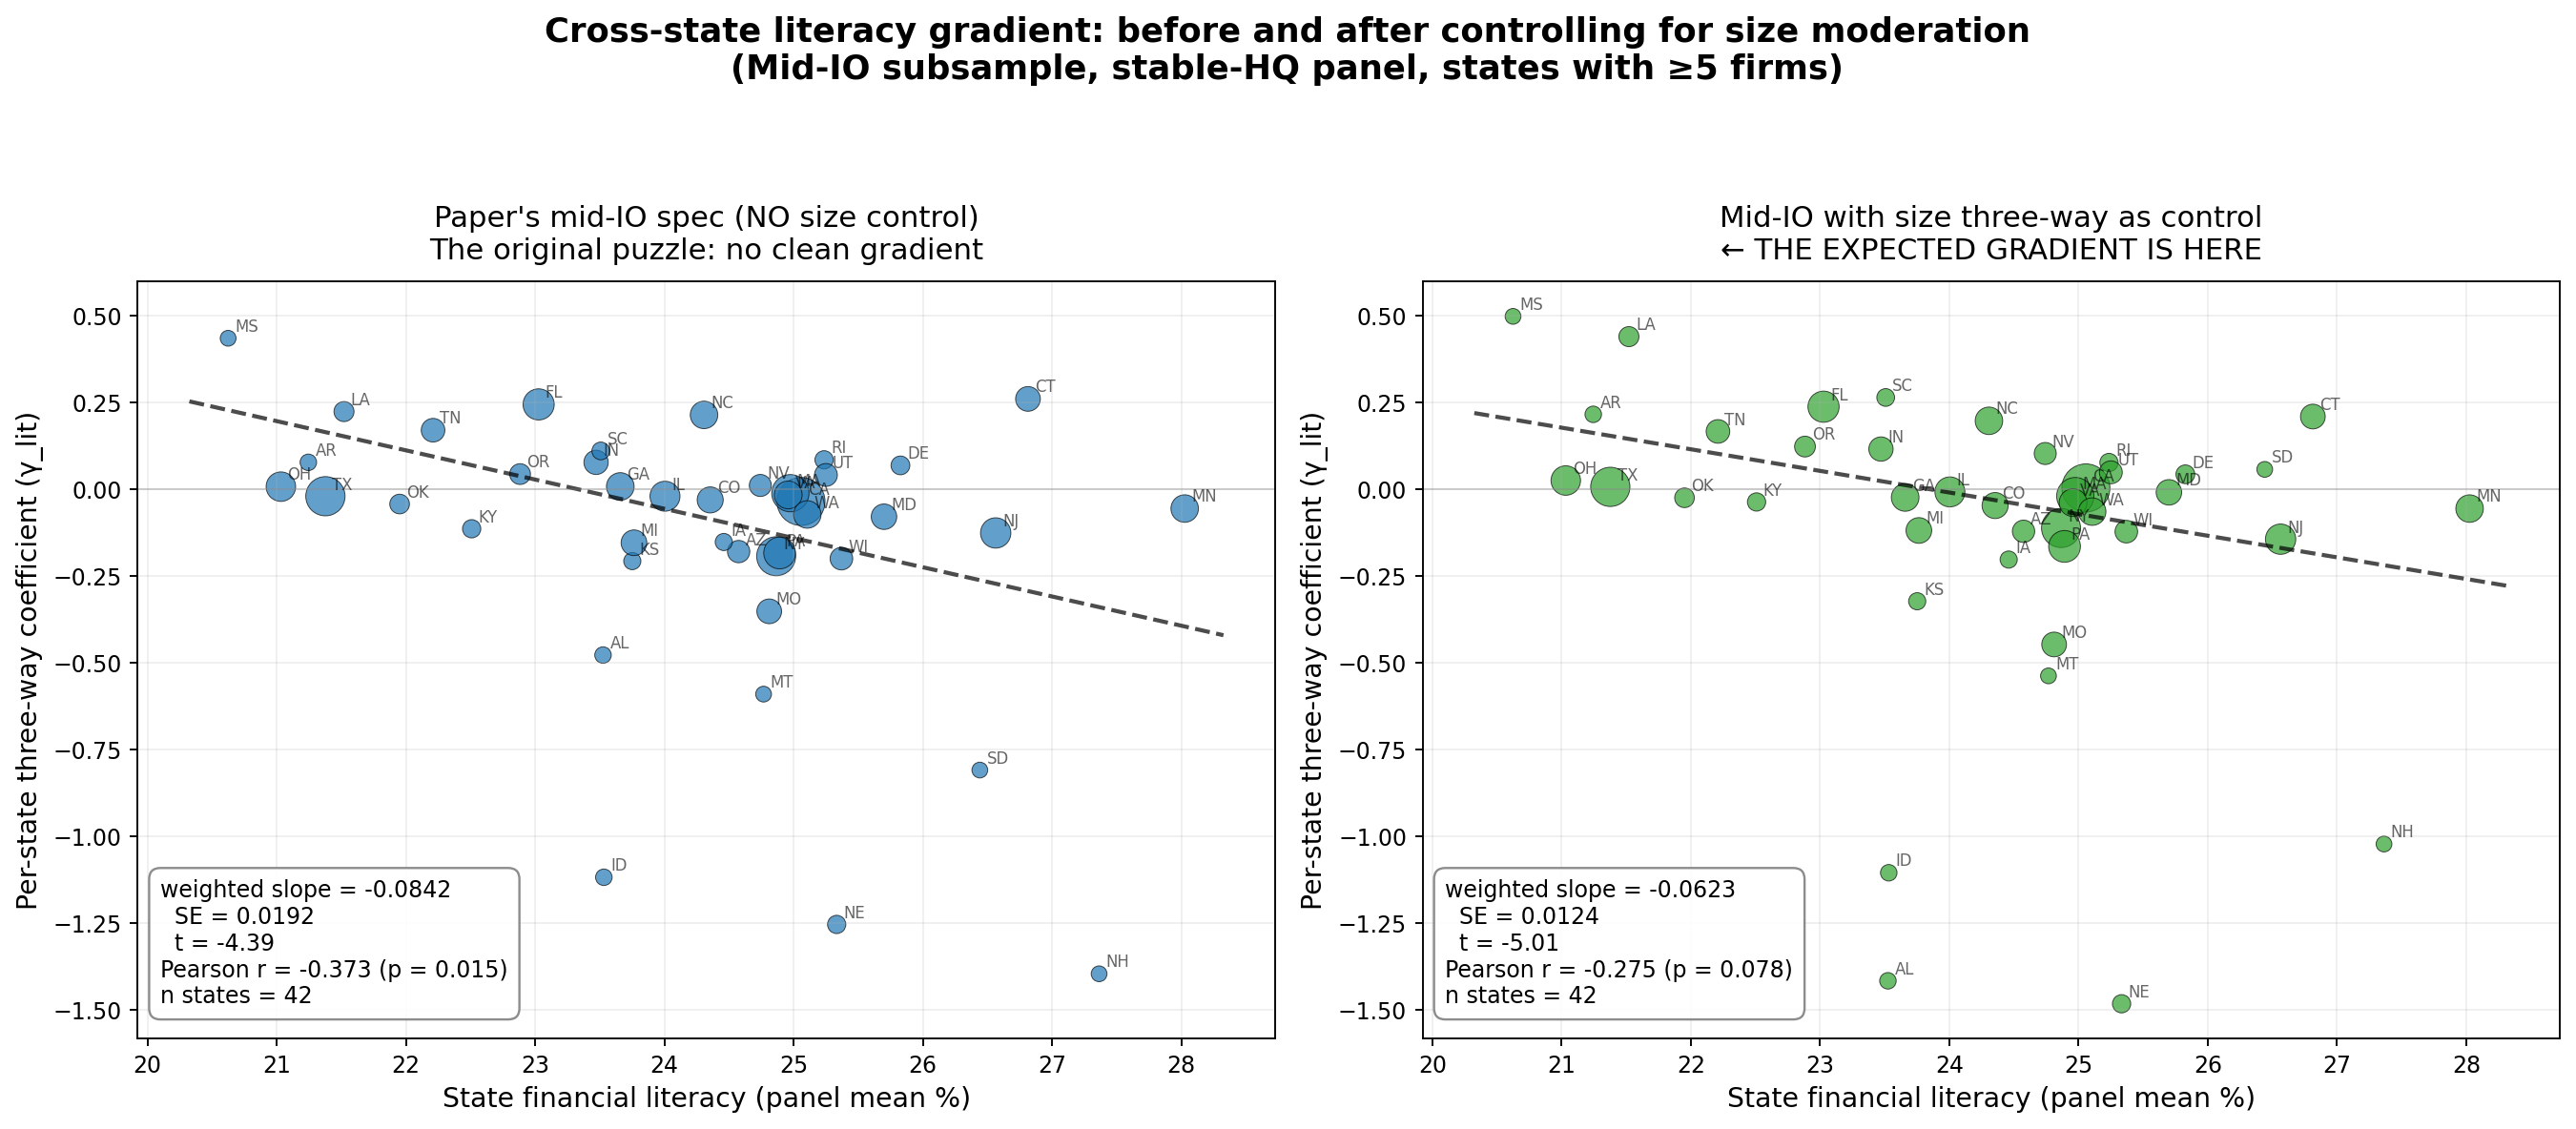
\includegraphics[width=\textwidth]{figures/punchline_size_controlled.png}
\caption{Cross-state literacy gradient under the size-controlled specification, full-panel mid-IO sample (left) and after dropping micro-caps (right). Point size $\propto \sqrt{n_{\text{firms}}}$; line is the precision-weighted slope.}
\label{fig:cross_state}
\end{figure}

\begin{figure}[h]
\centering
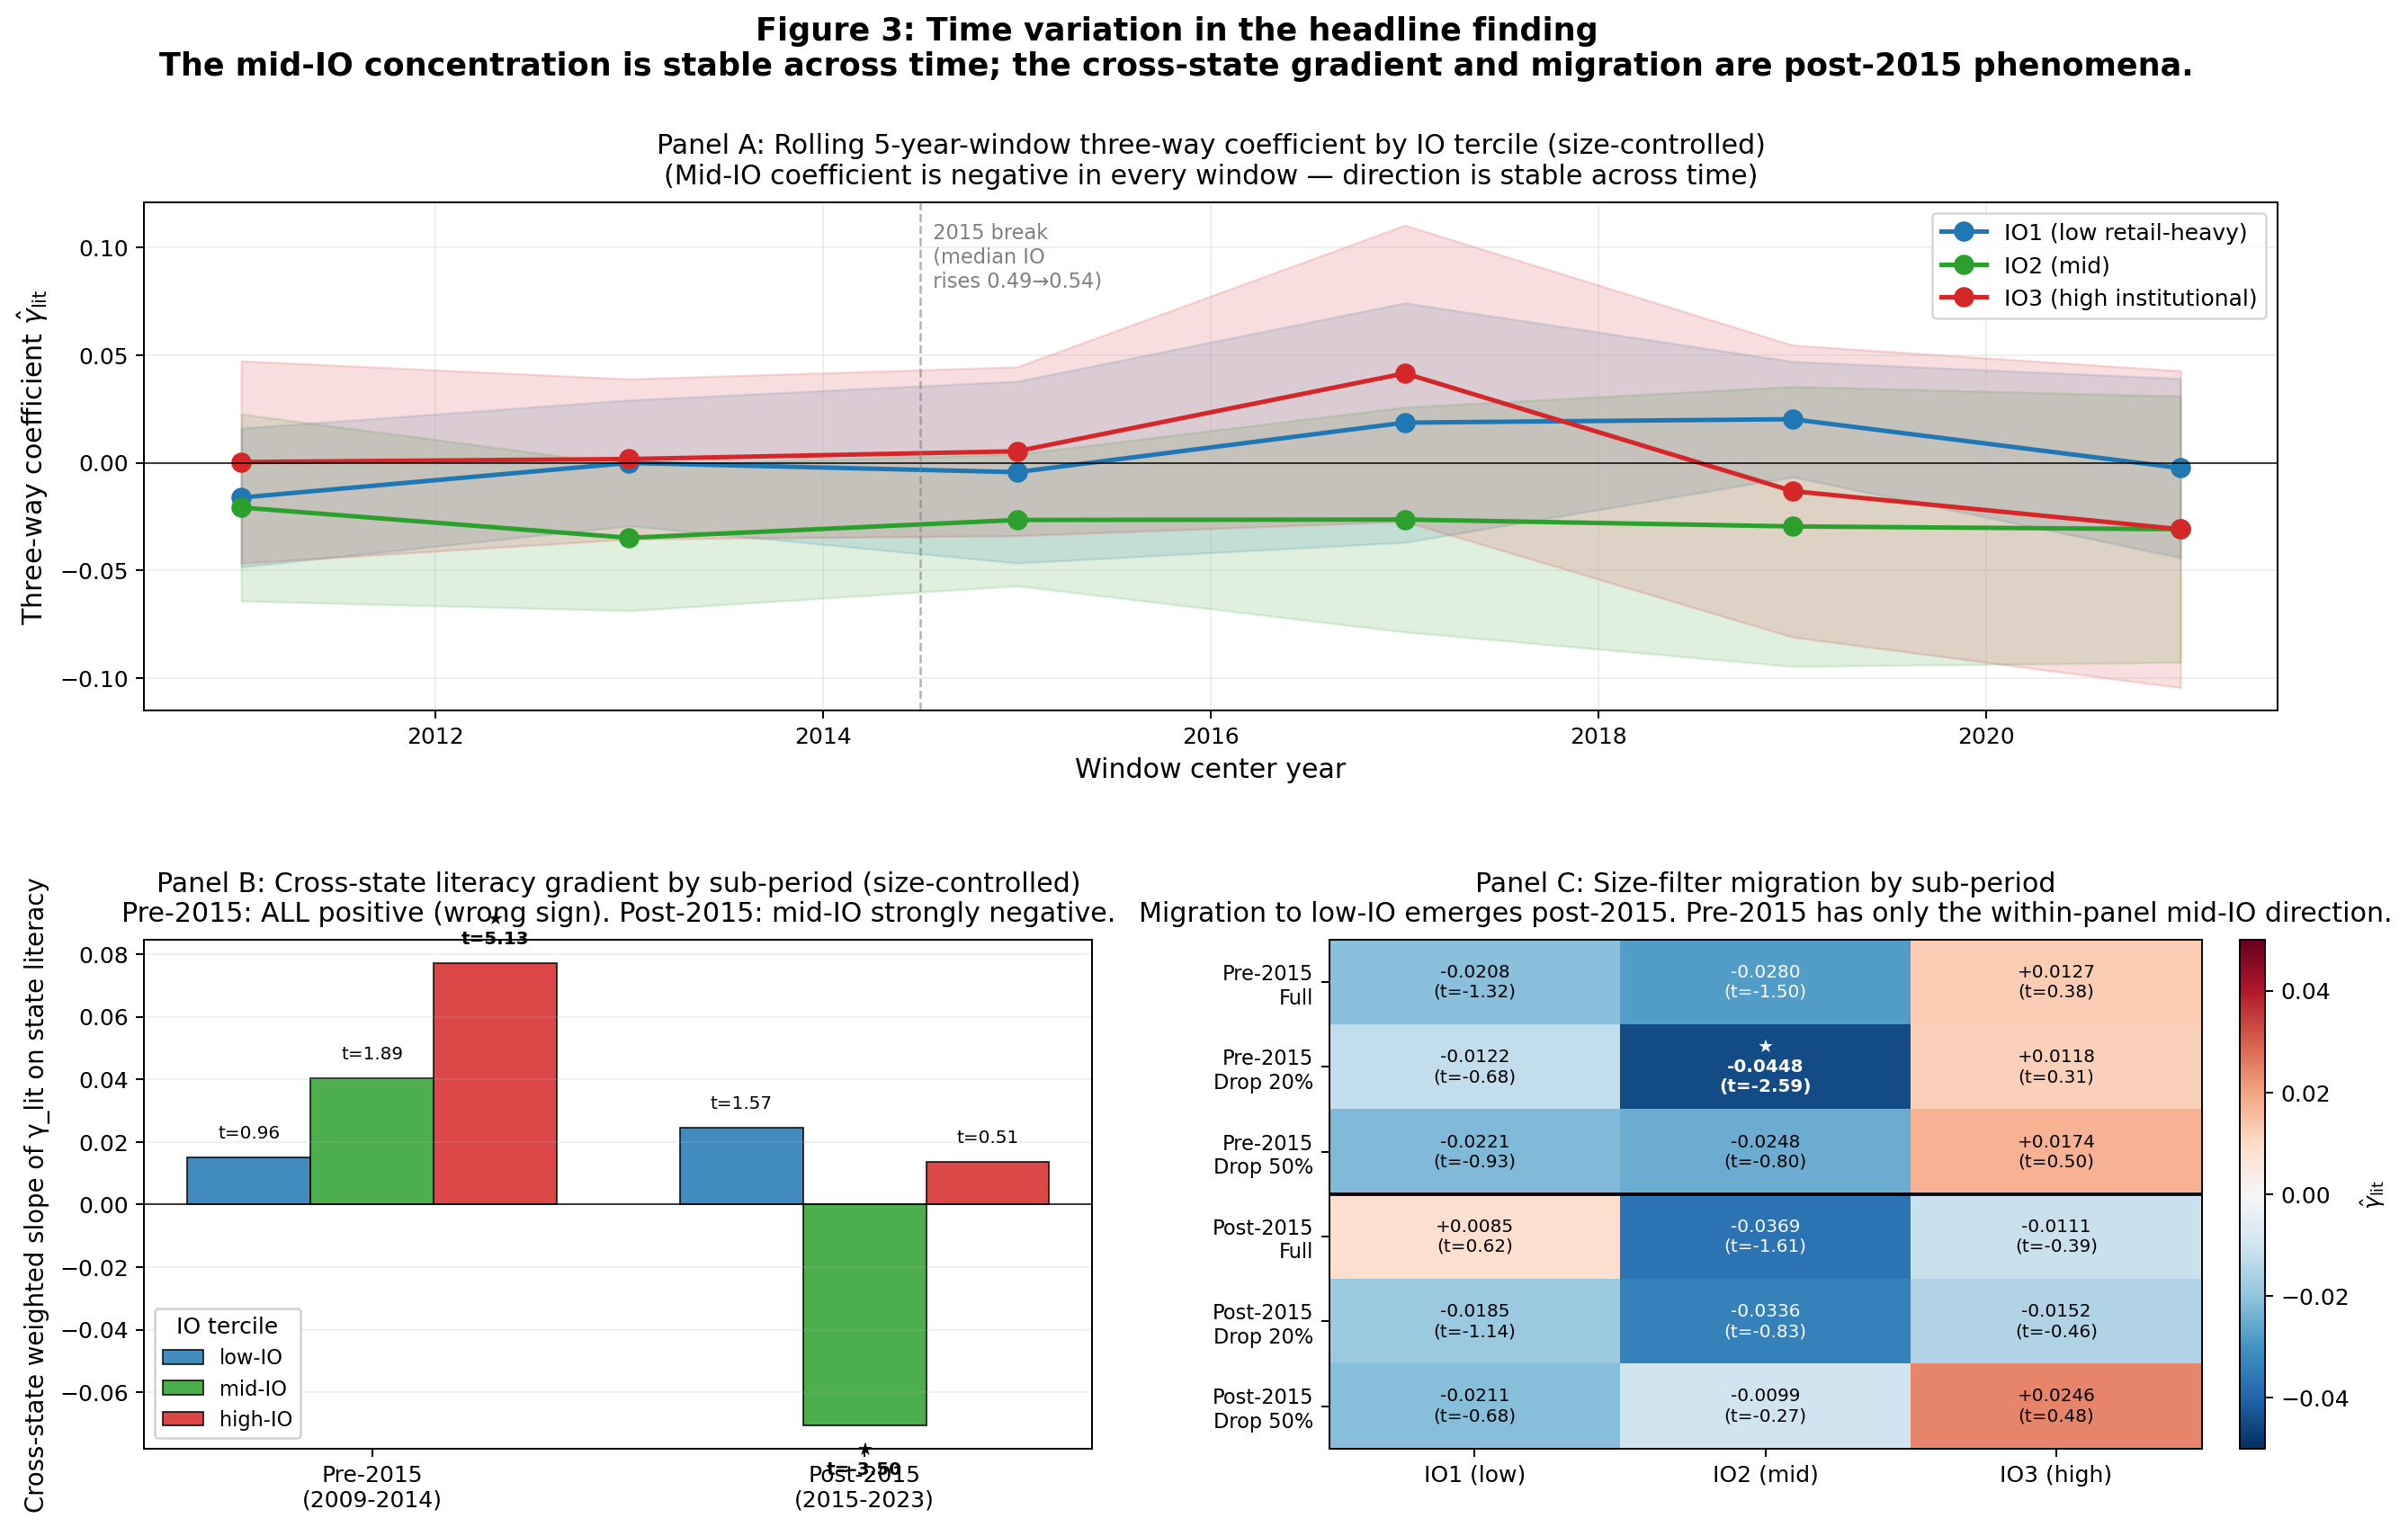
\includegraphics[width=\textwidth]{figures/figure3_time.png}
\caption{Time variation in the headline finding. Panel A: rolling 5-year-window mid-IO three-way coefficient is negative in every window. Panel B: cross-state literacy gradient by sub-period --- pre-2015 cells are wrong-signed, post-2015 cells are right-signed. Panel C: size-filter migration heatmap by sub-period.}
\label{fig:time}
\end{figure}

\bibliographystyle{plainnat}
\IfFileExists{references.bib}{\bibliography{references}}{}

\end{document}
